% DAC 2027 Research Track submission (double-blind). IEEE conference template, 6 pages + 1 page of references.
% Every number in tables/ and tables/numbers.tex is generated by gen_tables.py from the logged runs.
\documentclass[conference,10pt]{IEEEtran}
\IEEEoverridecommandlockouts
\usepackage[T1]{fontenc}
\usepackage{newtxtext,newtxmath}
\usepackage{cite}
\usepackage{amsmath}
\usepackage{graphicx}
\usepackage{booktabs}
\usepackage{multirow}
\usepackage{xcolor}
\usepackage{pifont}
\usepackage{listings}
\usepackage{tikz}
\usetikzlibrary{positioning,arrows.meta,fit,calc}
\usepackage[hidelinks,pdfauthor={},pdftitle={},pdfcreator={},pdfproducer={}]{hyperref}

\newcommand{\cmark}{\ding{51}}
\newcommand{\xmark}{\ding{55}}
\newcommand{\aegis}{\textsc{Aegis}}
% Visible marker for text that must be updated when the remaining runs finish. Remove before submission.
\newcommand{\pend}[1]{\textcolor{red}{[#1]}}
% generated by gen_tables.py -- do not edit
\newcommand{\AvgTAegis}{+18.8}
\newcommand{\AvgTDrrtl}{+13.9}
\newcommand{\AvgTVanilla}{+85.7}
\newcommand{\AvgWAegis}{+7.6}
\newcommand{\AvgWDrrtl}{+16.7}
\newcommand{\AvgWVanilla}{+87.2}
\newcommand{\MetaDrMax}{1,583}
\newcommand{\MetaDrMin}{1,430}
\newcommand{\MetaDrPct}{38}
\newcommand{\MetaNoInjTorn}{0}
\newcommand{\MetaOrigTorn}{0}
\newcommand{\MetaSeeds}{10}
\newcommand{\MetaWords}{4000}
\newcommand{\MetaWrites}{2000}
\newcommand{\MutChecker}{v1}
\newcommand{\NMcContractDesigns}{5}
\newcommand{\NMcDesigns}{9}
\newcommand{\NMcGrayDesigns}{6}
\newcommand{\NMcRunsDone}{12}
\newcommand{\NMcRunsTotal}{18}
\newcommand{\NMutBinaryCross}{21}
\newcommand{\NMutBinaryCrossEqyPass}{0}
\newcommand{\NMutBinaryCrossSimPass}{16}
\newcommand{\NMutContractNew}{0}
\newcommand{\NMutDesigns}{9}
\newcommand{\NMutExclDesigns}{6}
\newcommand{\NMutLabeled}{249}
\newcommand{\NMutSafe}{104}
\newcommand{\NMutSafeFalseAlarm}{0}
\newcommand{\NMutUnsafe}{127}
\newcommand{\NMutUnsafeBothPass}{1}
\newcommand{\NMutUnsafeCaught}{124}
\newcommand{\NMutUnsafeEqyPass}{27}
\newcommand{\NMutUnsafeSimPass}{19}
\newcommand{\NMutUnsafeStructMiss}{3}
\newcommand{\NMutUsed}{231}
\newcommand{\NScDesigns}{6}
\newcommand{\NScDoneAegis}{2}
\newcommand{\NScDoneDrrtl}{1}
\newcommand{\NScDoneVanilla}{3}
\newcommand{\NTokPairs}{6}
\newcommand{\ShipTAegis}{+18.8}
\newcommand{\ShipTDrrtl}{+12.8}
\newcommand{\ShipTVanilla}{+0.0}
\newcommand{\ShipWAegis}{+7.6}
\newcommand{\ShipWDrrtl}{+16.7}
\newcommand{\ShipWVanilla}{+0.0}
\newcommand{\TokRatioMedian}{2.2}

\makeatletter\let\tabinput\@@input\makeatother % plain \input breaks \bottomrule in tabulars

\lstset{basicstyle=\ttfamily\scriptsize,columns=fullflexible,keepspaces=true,frame=single,framesep=1pt,
  xleftmargin=2pt,xrightmargin=2pt,aboveskip=3pt,belowskip=0pt,commentstyle=\color{gray}}

\begin{document}

\title{\aegis: Clock-Domain-Aware Guardrails for\\Agentic LLM Timing Optimization of Multi-Clock RTL}
\author{\IEEEauthorblockN{Anonymous Author(s)}\IEEEauthorblockA{Submission ID: \pend{xxx}}}
\maketitle

\begin{abstract}
LLM agents now improve RTL timing by iterating rewrite, synthesis and equivalence checking. That correctness gate
is unsound for multi-clock designs: sequential equivalence and simulation reason about clean 0/1 values, so a
rewrite that breaks a clock-domain crossing (CDC) can pass both. Reproducing a state-of-the-art agent in an
open-source flow, we observe exactly this. On an AXI-Lite clock-domain bridge, it promotes a rewrite that duplicates
a synchronizer stage five times. The rewrite is formally equivalent and shows zero simulation mismatches, yet it can
tear a bus transaction in silicon. We present \aegis{}, which (i) recovers clock domains and classifies every
crossing on the elaborated netlist, (ii) locks what its verifiers cannot check with checksums that survive code
motion, (iii) selects optimization regions per clock domain and scores candidates with a period-normalized
objective, and (iv) re-classifies crossings and re-proves CDC contracts on every candidate. On a CDC mutation
benchmark, the re-check rejects \NMutUnsafeCaught{} of \NMutUnsafe{} CDC-unsafe mutants with no
false alarm on \NMutSafe{} safe ones. On \NMcDesigns{} open-source multi-clock designs, \aegis{} never promotes a
CDC-unsafe design. It uses a median \TokRatioMedian$\times$ fewer LLM tokens than the reproduced agent.
\pend{update with final Exp.~02/01 numbers}
\end{abstract}

\begin{IEEEkeywords}
RTL optimization, LLM agents, clock-domain crossing, formal equivalence, timing closure
\end{IEEEkeywords}

% =====================================================================================================
\section{Introduction}

Timing closure is one of the most labor-intensive stages of digital design. An engineer reads a timing report,
restructures the offending RTL, re-synthesizes, and repeats. A line of recent work automates this loop with large
language models (LLMs). RTLRewriter searches LLM-proposed rewrites with cost-aware Monte Carlo tree
search~\cite{rtlrewriter2024}. SymRTLO adds symbolic rewrite rules~\cite{symrtlo2025}. Dr.\,RTL closes the loop with
a multi-agent framework and a self-improving library of optimization skills~\cite{drrtl2026}. ARES adapts the
reasoning effort of such an agent to cut its cost~\cite{ares2027}. All of them share one correctness strategy: a
rewrite is accepted only if simulation and/or sequential equivalence checking (SEC) show it is equivalent to the
original. All of them are evaluated on single-clock designs.

That strategy is sound for single-clock logic but not, without qualification, for designs with asynchronous
clock-domain crossings. SEC and zero-delay simulation model every register as holding a clean 0 or
1~\cite{eqy}. Metastability, glitches on a crossing, and the multi-bit skew that Gray coding exists to tolerate are
invisible to both. A rewrite can therefore pass every gate these frameworks apply while breaking a crossing.
\textbf{This is not hypothetical.} We ported Dr.\,RTL's released agents and skill library to an open-source flow
and ran them on an AXI-Lite clock-domain bridge~\cite{forencich}. Its first iteration promoted the rewrite in
Fig.~\ref{fig:axil}. To reduce fan-out, it copies the second stage of a two-flop synchronizer five times, one copy per
group of captured bits. The copies are identical in zero-delay logic, so EQY proves the design equivalent and
differential simulation finds no mismatch. In silicon the first stage can be metastable, the five copies can resolve
differently, and the bridge can capture half of a new address with half of an old one. Duplicating synchronizer
flops is a textbook CDC error~\cite{cummings2008cdc}. Even the benchmarks reflect the blind spot: Dr.\,RTL's
two-clock FIFO clocks every ``synchronizer'' in the \emph{source} domain, so all of its cross-domain paths are
unsynchronized (Sec.~\ref{sec:setup}). Single-clock synthesis neither times nor checks those paths.

\begin{figure}[t]
\begin{lstlisting}[language=Verilog]
// original: one 2-flop synchronizer qualifies the AXI-Lite write
s_flag_sync_reg_1 <= s_flag_reg;
s_flag_sync_reg_2 <= s_flag_sync_reg_1;
// promoted rewrite (EQY: PASS, simulation: 0 mismatches)
s_flag_sync_reg_2_aa_lo <= s_flag_sync_reg_1; // addr, low half
s_flag_sync_reg_2_aa_hi <= s_flag_sync_reg_1; // addr, high half
s_flag_sync_reg_2_wd_lo <= s_flag_sync_reg_1; // data, low (+2 more)
if (ld_aa_lo) m_axil_awaddr_reg[ADDR_HALF-1:0] <= ...;
\end{lstlisting}
\vspace{-2pt}
\caption{A CDC-unsafe rewrite accepted by an SEC-gated LLM optimizer (\texttt{axil\_cdc}, reproduced Dr.\,RTL,
iteration~1). \aegis{} rejects it twice: the lock checksum on the synchronizer and the CDC re-check, which finds the
synchronizer and four qualified captures downgraded.}
\label{fig:axil}
\vspace{-8pt}
\end{figure}

\aegis{} treats CDC correctness as a separate obligation from functional equivalence. Its contributions are:
\begin{itemize}
\item \textbf{A netlist-level CDC shield} for LLM optimization. Crossings are classified on the elaborated design,
  and logic falls into three lock tiers (immutable, contract-bound, free). Checksums that survive code motion
  enforce the locks before any simulation or formal effort is spent.
\item \textbf{A post-generation CDC re-check.} Every candidate is re-classified, and the CDC contracts proven on the
  baseline (Gray stepping, handshake stability, registered launch) are re-proven with SymbiYosys at their
  calibrated latency. This catches rewrites that are equivalent but CDC-unsafe.
\item \textbf{Multi-clock optimization.} Optimization targets are regions of overlapping logic cones, selected with
  per-domain quotas. Candidates are scored per domain, with deficits normalized by each domain's own period.
\item \textbf{An open evaluation} on \NMcDesigns{} multi-clock designs plus \NScDesigns{} of Dr.\,RTL's designs. It compares
  against a reproduction of Dr.\,RTL and an unguarded LLM baseline under one open-source flow, and adds a CDC
  mutation benchmark with known ground truth.
\end{itemize}

% =====================================================================================================
\section{Background and Related Work}

\textbf{CDC.} A signal crossing between asynchronous clocks can violate the receiving flip-flop's setup or hold
window and go metastable. Single-bit crossings are protected by a synchronizer, a chain of two or more destination
flops with no logic between them. Multi-bit values cross as Gray codes, where one bit changes per step so a skewed
sample is still a neighbor value, or under a handshake that keeps the data stable while it is sampled. Each scheme
has a \emph{structural} part (registered launch, no logic in the chain) and a \emph{protocol} part (one-bit
stepping, stability). Neither is visible to zero-delay simulation~\cite{mvcdc2024} or to SEC, which in Yosys models
multiple clocks as sampled transitions of one global clock~\cite{eqy}. Industrial CDC tools add convergence
analysis, protocol checks and metastability injection~\cite{li2009cdc,mvcdc2024}. Open-source CDC tooling is far
less mature~\cite{vygescdc,opencdc}.

\textbf{LLM RTL optimization.} RTLRewriter~\cite{rtlrewriter2024}, SymRTLO~\cite{symrtlo2025},
VeriOpt~\cite{veriopt2025}, ASPEN~\cite{aspen2025}, Dr.\,RTL~\cite{drrtl2026} and ARES~\cite{ares2027} optimize
single-clock RTL, gated by simulation or SEC. RTL-OPT~\cite{rtlopt2026} pairs single-clock designs with optimized
references. Xu et al.~\cite{xu2025} include 32 clock-domain cases, made by splitting single-clock logic across
domains. They measure only PPA, not CDC correctness, and find that LLMs do no better than Yosys on those cases. CDC
mutation operators exist as a patented method without a dataset~\cite{gupta2018cdcmutation}. Benchmarks for RTL
bugs~\cite{mantra2023,veribugbench2026,gatetruth2026} target functional bugs. To our knowledge, no LLM optimizer
protects crossings during optimization, and no prior evaluation checks whether optimized multi-clock designs remain
CDC-safe.

% =====================================================================================================
\section{The \aegis{} Framework}
\label{sec:method}

\begin{figure}[t]
\centering
\resizebox{\columnwidth}{!}{%
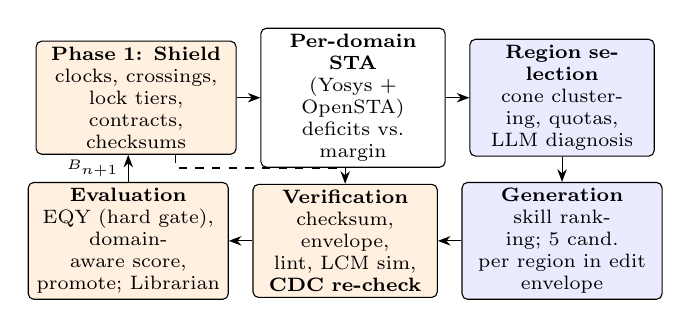
\begin{tikzpicture}[font=\scriptsize, node distance=3.2mm and 3mm,
  box/.style={draw, rounded corners=2pt, align=center, minimum height=8mm, inner sep=2pt, text width=#1},
  box/.default=19mm, llm/.style={box=#1, fill=blue!8}, llm/.default=19mm,
  gate/.style={box=#1, fill=orange!12}, gate/.default=19mm, arr/.style={-{Stealth[length=1.6mm]}}]
\node[gate=24mm] (p1) {\textbf{Phase 1: Shield}\\clocks, crossings,\\lock tiers, contracts,\\checksums};
\node[box=22mm, right=of p1] (sta) {\textbf{Per-domain STA}\\(Yosys + OpenSTA)\\deficits vs.\ margin};
\node[llm=22mm, right=of sta] (sel) {\textbf{Region selection}\\cone clustering, quotas,\\LLM diagnosis};
\node[llm=24mm, below=of sel] (gen) {\textbf{Generation}\\skill ranking; 5 cand.\\per region in edit\\envelope};
\node[gate=22mm, left=of gen] (ver) {\textbf{Verification}\\checksum, envelope,\\lint, LCM sim,\\\textbf{CDC re-check}};
\node[gate=24mm, left=of ver] (ev) {\textbf{Evaluation}\\EQY (hard gate),\\domain-aware score,\\promote; Librarian};
\draw[arr] (p1) -- (sta); \draw[arr] (sta) -- (sel); \draw[arr] (sel) -- (gen); \draw[arr] (gen) -- (ver);
\draw[arr] (ver) -- (ev); \draw[arr] (ev.north) -- node[left, align=right, font=\tiny]{$B_{n+1}$} (p1.south -| ev.north) ;
\draw[arr, dashed] (p1.south) ++(5mm,0) |- ($(ver.north)+(0,2mm)$) -- (ver.north);
\end{tikzpicture}}
\vspace{-4pt}
\caption{\aegis{} loop. Orange: deterministic gates that the LLM cannot bypass. Blue: steps that call the LLM.
The dashed edge shows locks and contracts from Phase~1 being re-checked on every candidate.}
\label{fig:flow}
\vspace{-8pt}
\end{figure}

\aegis{} (Fig.~\ref{fig:flow}) keeps the closed loop of agentic optimizers but changes three things. Every safety
invariant is enforced by deterministic code, not by prompting. The loop reasons per clock domain. And CDC safety is
checked separately from equivalence. The LLM is called only for region diagnosis, skill ranking and candidate RTL.
The orchestrator, gates, promotion and termination are about 4{,}000 lines of Python around Yosys~\cite{yosys},
OpenSTA~\cite{opensta}, SymbiYosys~\cite{sby} and EQY~\cite{eqy}.

\subsection{Phase 1: The CDC Shield}
\label{sec:phase1}

\textbf{Clocks and constraints.} \aegis{} parses the SDC into master and generated clocks and classifies every
clock pair as identical, related (same master), or asynchronous. Asynchronous pairs that are neither declared
exclusive nor bounded with \texttt{set\_max\_delay -datapath\_only} are written to a constraint-audit report. A
violation on an asynchronous path is a constraint issue, not an RTL timing defect, so it is never sent to the
optimizer.

\textbf{Crossings.} Crossings are found on the elaborated, flattened netlist (Yosys \texttt{proc; flatten;
opt\_dff}), so hierarchy and coding style do not matter. \texttt{opt\_dff} folds resets and enables into the flop,
so a reset multiplexer cannot hide a direct flop-to-flop connection. Each flop is assigned its SDC clock, and its
combinational fan-in is traced back to source flops. A source in an asynchronous domain makes a crossing, which is
classified as a \emph{synchronizer} (direct connection followed by at least one more same-domain stage), a
\emph{Gray candidate} (multi-bit synchronizer), a \emph{qualified capture} (data loaded under a synchronized
enable), \emph{insufficient depth}, or \emph{unsynchronized}. The last two are reported as pre-existing issues.
\aegis{} still optimizes such designs, but never makes the classification worse.

\textbf{Lock tiers.} Every source statement falls into one of three tiers.
\emph{Immutable} covers synchronizer blocks, \texttt{ASYNC\_REG}/\texttt{keep} flops, clock dividers (whose ratios
the SDC depends on), parameters, the launch and capture registers of every crossing that has no proven contract,
and, for such Gray crossings, the whole fan-in of the launch register. Without that last rule, an LLM could turn the
next-Gray-value logic into a binary increment while leaving the locked register untouched.
\emph{Contract-bound} covers the fan-in of crossings whose CDC contract is proven on the baseline.
\emph{Free} is everything else. A contract is a set of single-clock properties instantiated from templates around
the crossing's module and proven with SymbiYosys (PDR, then $k$-induction). The launch register need not be a port:
\aegis{} elaborates the module at its instance parameters, exposes the register as an output with Yosys, and prunes
the netlist to that register's fan-in cone, so a FIFO's memory and data path do not enter the proof. When the launch
flop has no direct reset (e.g., a reset synchronizer drives it), every reset input of the module gates the
properties, with a settle window after release. G1/G2 state that the pointer changes
by at most one bit, and only on an increment. H1--H3 state that data is stable while a request is pending. R4
requires a registered launch, because a combinational launch can glitch and no value-level property sees a glitch.
Latency-parameterized templates are \emph{calibrated}: the smallest latency at which the contract holds on the
baseline is recorded, and candidates must prove it at that latency.

\textbf{Checksums.} For each immutable register, \aegis{} stores a SHA-256 digest of its normalized source,
without line numbers. To check a candidate, it re-elaborates it, finds each locked register through Yosys
source-location attributes, and recomputes the digest. Code inserted or moved elsewhere leaves every digest
unchanged. A missing register, a changed digest, or a touched SDC rejects the candidate before any lint, simulation
or formal compute, so compliance does not rely on the LLM reporting it.

\subsection{Per-Domain Region Selection}

Prior agents rank a global list of paths by slack~\cite{drrtl2026}. In a multi-clock design this fails three ways.
Nanoseconds are not comparable across periods. One domain's near-critical paths can starve the others. And many
paths through one multiplier are one problem, not many. \aegis{} runs OpenSTA per capture clock and computes each
endpoint's deficit against a closure margin $m$, $\delta_e=\max(0,m-s_e)$. It drops asynchronous endpoints, maps
each remaining endpoint to its RTL register (via Yosys source attributes, else by normalized name), and computes its
combinational fan-in cone of source statements. Endpoints whose cone lies entirely in locked logic are recorded as
\emph{blocked}, which is the measurable cost of the guardrail.

Endpoints of one domain are clustered into \emph{regions} with union-find wherever their cones' overlap
coefficient $|C_i\cap C_j|/\min(|C_i|,|C_j|)$ reaches $\theta$. Control nets with fan-out above $\varphi$ are
ignored for this test only, and regions are capped in size so each fits one prompt. One LLM call per region assigns
each endpoint a root cause and an amenability label (combinational, sequential-safe, sequential-unsafe, or out of
scope). Region $r$ in domain $d$ is scored
$P_r=\alpha\,\Delta^{\max}_r/\Delta^{\max}_d+\beta\,\Delta^{\Sigma}_r/\Delta^{\Sigma}_d$ over its amenable
endpoints. A budget of $B$ regions is split so that every violating domain gets one slot and the rest go in
proportion to $w_d\Delta^{\Sigma}_d$, where $w_d=f_d/f_{\max}$. Up to three pairwise-disjoint regions are dispatched
per iteration. A region that fails twice becomes tabu.

\subsection{Generation and Verification}

For each region, a skill library keyed by root cause supplies the eligible skills. It has 65 entries: Dr.\,RTL's 47
published skills~\cite{drrtl2026} plus 18 of ours, including CDC contract-bound skills and ``do not use'' entries
that describe CDC-breaking rewrites. The LLM ranks the eligible entries. Five candidates are generated: two from the
top skill, two from the second, and one latency-preserving rewrite with no skill. Each may change only lines inside
the region's \emph{edit envelope}, its editable cones plus the always-blocks that assign its endpoints, minus locked
logic. The envelope is enforced by a normalized line diff, and port lists and the module set must be unchanged.

Candidates then pass a cascade that stops at the first failure: (1)~checksum and envelope gate; (2)~lint (Icarus,
Verilator); (3)~\emph{LCM multi-clock differential simulation}, which drives every clock at its SDC period with
input changes off clock edges, over $\max(4\cdot\mathrm{LCM},200\,T_{\max})$ for two seeds; and (4)~the \emph{CDC
re-check}. The re-check re-runs Phase~1 on the candidate. It rejects any new unsynchronized or insufficient-depth
crossing, any baseline synchronizer, Gray or qualified crossing that disappears or loses depth, and any baseline
contract that no longer proves at its calibrated latency. Phase~1 does not classify reads of a memory as crossings:
FIFO storage is protected by the pointer protocol, which the Gray contracts and synchronizer checks cover. A rewrite
that recodes an original memory as an array of registers gets the same treatment, so its entries are recorded, not
counted as new crossings. Survivors must pass EQY against the current baseline on
every module they touch; FAIL, ERROR and timeout all disqualify.

\subsection{Domain-Aware Scoring and Promotion}

Dr.\,RTL scores a candidate as $0.5\,\mathrm{WNS}^{n}+0.35\,\mathrm{TNS}^{n}+0.15\,\mathrm{Area}^{n}$ over the
whole design~\cite{drrtl2026}. That can hide a fast domain's regression behind a slow domain's gain. \aegis{} scores
\begin{gather*}
S=\frac{\sum_d w_d(\alpha W_d+\beta T_d)}{\sum_d w_d}+\gamma f(A),\\
W_d=\frac{D^{\max}_d-\hat D^{\max}_d}{\max(\hat D^{\max}_d,\;0.01\,T^{clk}_d)}.
\end{gather*}
Here $\hat D$ is the baseline's deficit, $T_d$ is defined like $W_d$ on total deficit, and $f(A)$ is the relative
area change with a quadratic penalty above $+5\%$. An adaptive schedule moves weight from worst to total deficit,
and to area once every domain meets the margin. Winners of disjoint regions are composed when the composition
scores better. The iteration winner replaces the baseline only if $S<0$. In the last iteration, a winner that
worsens any domain's worst deficit is rejected. A Librarian updates skill confidences from group-relative
advantages and quotes recent rejection reasons in later prompts. The loop stops after five iterations or when
nothing is dispatchable. (An optional rule also stops after two iterations with gains below $10^{-3}$; we disable it
in all experiments so that every method gets the same budget.)

% =====================================================================================================
\section{Experimental Setup}
\label{sec:setup}

\textbf{Designs.} The multi-clock suite (Table~\ref{tab:suite}) has \NMcDesigns{} designs with 2--4 clocks:
asynchronous FIFOs from four independent code bases~\cite{dpretet,wb2axip,opentitan,commoncells}, an AXI-Stream
frame FIFO, an AXI-Lite bridge and a three-clock Ethernet MAC~\cite{forencich}, Dr.\,RTL's FIFO constrained with
both of its clocks, and \texttt{soc}, a four-clock test system we wrote with two deliberately unsynchronized
crossings. Each domain's period is set to 75\% of its critical-path delay under the raw flow, so every domain
violates. The single-clock suite is the \NScDesigns{} smallest (by baseline area) of Dr.\,RTL's 20 released
designs, at its 0.1\,ns clock; we chose the subset by size alone, before seeing any result, to bound LLM cost.

\begin{table}[t]
\centering
\caption{Multi-clock suite: Phase~1 crossing classification and the synthesis-only baseline (Nangate45; ns,
$\mu$m$^2$). Unsync.\ includes insufficient depth.}
\label{tab:suite}
\vspace{-4pt}
\setlength{\tabcolsep}{2.2pt}
\scriptsize
\begin{tabular}{@{}lrrrrrrrrrr@{}}
\toprule
Design & Clk & FF & Sync & Gray & Qual. & Unsync. & Contr. & WNS & TNS & Area\\
\midrule
\tabinput tables/suite.tex 
\bottomrule
\end{tabular}
\vspace{-8pt}
\end{table}

Phase~1 finds exactly the two crossings left unsynchronized in \texttt{soc}, and none in the six third-party
FIFOs and bridges. On \texttt{drrtl\_fifo\_2clk} it reports 142 unsynchronized crossings and
no synchronizer. Dr.\,RTL's FIFO registers each pointer twice, but in the \emph{source} domain. On
\texttt{cc\_cdc\_fifo\_gray} it reports 9 unsynchronized crossings because it does not recognize the PULP
library's synchronizer cell, a known false positive.
Gray contracts are proven automatically on \NMcContractDesigns{} of the \NMcGrayDesigns{} designs with Gray
crossings (column Contr.); where none proves, the Gray logic stays immutable. \pend{check after the Phase~1 re-run}

\textbf{Flow.} All configurations are measured in one flow: Yosys~0.67 with a timing-driven ABC script on
Nangate45~\cite{nangate45}, then OpenSTA. Reported gains are therefore gains over what synthesis finds by itself.
Final designs are checked against the \emph{original} RTL with EQY on the top module and with the CDC re-check,
whatever the configuration.

\textbf{Configurations.} All use Claude Sonnet~5.5 through the same command-line interface, with five iterations of five candidates (Dr.\,RTL: five per major version). \emph{Vanilla} gives the
model the RTL and its timing report, with no locks, skills, envelope or gating except synthesizability, and
promotes the best-scoring candidate. Every guardrail is still \emph{measured}. \emph{Dr.\,RTL (reproduced)} runs
Dr.\,RTL's released analyzer and optimizer prompts and skill library verbatim, with its loop and score. Only the
tools change: Design Compiler becomes Yosys+OpenSTA, and Jasper SEC becomes EQY against the original. Two
departures favor Dr.\,RTL. Its skill library was learned on its own 20 designs. And candidates that fail lint or
simulation still reach its SEC gate. We use five major iterations instead of its ten, to match budgets.
\aegis{} runs as described, without early stopping. Runs that lose candidates to account usage limits are
discarded and re-run. Each
configuration is run once per design \pend{repeats if time permits}.

% =====================================================================================================
\section{Results}

\subsection{Multi-Clock Optimization}

\begin{table*}[t]
\centering
\caption{Multi-clock results (one run each; Claude Sonnet; 5 iterations for every method). WNS is the worst
domain; percentages are improvements (positive = closer to zero). EQY and CDC refer to the final design vs.\ the
original RTL. n/c: nothing promoted. \textbf{?}: CDC re-check flags the final design, not audited by hand.
\emph{Shippable only}: a final design that fails EQY or is CDC-unsafe counts as 0\%, since it cannot be used.
Flat: worst-domain WNS improvement when the original and final designs are both re-synthesized with the hierarchy
flattened (gains that rely on module boundaries vanish). CDC is re-measured on every final design with one checker.}
\label{tab:mc}
\vspace{-4pt}
\setlength{\tabcolsep}{5pt}
\footnotesize
\begin{tabular}{@{}llccrrcccr@{}}
\toprule
Design & Config & WNS (ns) & TNS (ns) & Flat\% & $\Delta$A\% & EQY & CDC & kTok & Calls\\
\midrule
\tabinput tables/multiclock.tex 
\bottomrule
\end{tabular}
\vspace{-10pt}
\end{table*}

Table~\ref{tab:mc} reports the \NMcRunsDone{} of \NMcRunsTotal{} \aegis{} and Dr.\,RTL runs completed so far.
\pend{The \aegis{} rows are still from the version before the contract and memory fixes of
Sec.~\ref{sec:phase1} and with early stopping; they are being re-run. Update this section when the runs finish.}
Four observations stand out.

\textbf{Unguarded gains are not real.} Vanilla meets timing on \texttt{afifo} and \texttt{prim\_fifo\_async} and
halves WNS on \texttt{soc}. None of its final designs passes EQY against the original, and on
\texttt{afifo} it reaches timing closure partly by reading the \emph{first} stage of a two-flop synchronizer
(depth $2\to1$), with zero simulation mismatches. The same holds on the single-clock suite
(Table~\ref{tab:sc}): no vanilla final design is proven equivalent, and two show simulation mismatches.

\textbf{SEC gating is not enough.} The reproduced Dr.\,RTL is held to EQY, and all its final designs pass. On
\texttt{axil\_cdc}, however, its final design is the rewrite of Fig.~\ref{fig:axil}. It bought 1.25\,ns of TNS by
duplicating a synchronizer stage. To check that the hazard is real, we simulate \MetaWrites{} random AXI-Lite writes
through both designs with metastability injection: in the cycle after a first synchronizer stage changes, every flop
that samples it independently sees the old or the new value (applied identically to every synchronizer). Without
injection both designs deliver every write intact, as EQY and simulation predict. With it, the original
corrupts \MetaOrigTorn{} words in \MetaSeeds{} seeds, while the rewrite corrupts \MetaDrMin--\MetaDrMax{} of
\MetaWords{} address and data words (${\approx}\MetaDrPct\%$): its five copies disagree and the bridge tears the
transaction. The injection is worst-case, so this shows the failure mode, not its rate in silicon. \aegis{}'s lock and CDC re-check reject this class of rewrite, and no final
\aegis{} design is CDC-unsafe.

\textbf{Timing is competitive, not dominant.} \pend{Rewrite after the \aegis{} re-runs; describes the old version.}
Where both methods finish, \aegis{} reaches a clearly better result on
\texttt{async\_fifo} (TNS $-2.87\to-0.58$ vs.\ $-2.19$\,ns), matches Dr.\,RTL on \texttt{soc} and
\texttt{prim\_fifo\_async}, and is behind on \texttt{axil\_cdc} (where Dr.\,RTL's gain is unsafe), on \texttt{afifo} and on
\texttt{axis\_async\_fifo}. On the last two, Dr.\,RTL's worst-domain gains ($-0.15\to+0.05$ and
$-0.24\to-0.11$\,ns) are CDC-safe by manual audit. \aegis{} could not reach them for two reasons. Without a proven
Gray contract, the pointer logic is immutable and the text-level checksum rejects equivalent restructurings of it.
And the structural re-check misreads a FIFO memory recoded as registers as new crossings, which is what flags both
Dr.\,RTL final designs (Sec.~\ref{sec:limits}).

\textbf{Cost.} Region-scoped prompts and no budget spent on asynchronous paths make \aegis{}
cheaper on every design where both runs exist \pend{re-check with the full-budget re-runs}: a median \TokRatioMedian$\times$ fewer tokens over \NTokPairs{}
designs, and $7.4\times$ fewer on \texttt{soc}. There, the reproduced Dr.\,RTL chose \texttt{soc}'s deliberately
unsynchronized path as the critical path in all five iterations, a path \aegis{} sends to the constraint audit.

\subsection{Single-Clock Suite}

\begin{table}[t]
\centering
\caption{The \NScDesigns{} smallest of Dr.\,RTL's single-clock designs: runs done, final designs that changed (promoted) and that pass EQY
vs.\ the original, and the median WNS/TNS improvement (\%) over EQY-passing final designs.}
\label{tab:sc}
\vspace{-4pt}
\scriptsize
\begin{tabular}{@{}lcccrr@{}}
\toprule
Config & Runs & Promoted & EQY pass & $\Delta$WNS\% & $\Delta$TNS\%\\
\midrule
\tabinput tables/singleclock.tex 
\bottomrule
\end{tabular}
\vspace{-8pt}
\end{table}

\pend{Exp.~01 is \NScDoneAegis/\NScDoneDrrtl/\NScDoneVanilla{} of \NScDesigns{} runs (\aegis/Dr.\,RTL/vanilla); write this
paragraph (does \aegis{}'s machinery cost it the single-clock case?) once it completes.}

\subsection{CDC Mutation Benchmark}

To measure which gate catches which fault, independently of any LLM, we inject CDC faults into the netlists of
multi-clock designs (the suite plus further bridges and PULP CDC cells) at every crossing Phase~1 found. Each mutant carries a ground-truth
CDC label. Unsafe operators bypass or remove a synchronizer stage, clock it from the wrong domain, re-encode a Gray
crossing in binary, or tie a capture qualifier active. Safe operators add a stage, invert a synchronized bit (a
functional bug), or are no-op controls. Of \NMutLabeled{} labeled mutants, we use \NMutUsed{} on \NMutDesigns{}
designs \pend{labeling in progress}. \NMutExclDesigns{} PULP designs are excluded because the structural check flags their identity controls
(the synchronizer cell is not recognized, Sec.~\ref{sec:setup}). EQY compares each mutant with the identity netlist.

\begin{table}[t]
\centering
\caption{CDC mutation benchmark: CDC-unsafe mutants rejected, and CDC-safe mutants flagged as CDC-unsafe.
Functional gates are expected to reject safe but non-equivalent mutants, so no false-alarm rate is given for them.}
\label{tab:mut}
\vspace{-4pt}
\scriptsize
\begin{tabular}{@{}lcc@{}}
\toprule
Check & Unsafe rejected & Safe flagged\\
\midrule
\tabinput tables/mutants.tex 
\bottomrule
\end{tabular}
\vspace{-8pt}
\end{table}

Table~\ref{tab:mut} shows the CDC re-check rejecting all but \NMutUnsafeStructMiss{} of \NMutUnsafe{} unsafe
mutants with no false alarm. Functional gates reject most unsafe mutants too, but for the wrong reason. Most of these
mutants change latency, so simulation sees a mismatch. EQY's ``failure'' is often a missing proof rather than a
counterexample. On the latency-preserving binary-Gray re-encoding, simulation passes
\NMutBinaryCrossSimPass{} of \NMutBinaryCross{}. The LLM rewrite of Fig.~\ref{fig:axil} is exactly such a
latency-preserving fault, and it passes both functional gates. The three misses are synchronizer removals on
\texttt{axis\_async\_fifo}'s status flags: the mutant replaces the last stage of a toggle synchronizer with a wire
to the source-domain register, so an unsynchronized signal reaches a top-level status output through an XOR. Phase~1
classifies flop-to-flop crossings only, and here the capturing flop lies outside the design. The new Gray contracts
add a second, independent detection to \NMutContractNew{} unsafe mutants the structural check already caught,
with no new false alarm.

% =====================================================================================================
\section{Limitations}
\label{sec:limits}

\aegis{} guarantees that optimization never makes a design's CDC status worse \emph{as measured by} its
structural classification and proven contracts. It is not sign-off CDC: it does no convergence analysis or
metastability injection. Locks are text-level fingerprints, so they also reject equivalent restructurings of locked
logic; this matters wherever a crossing has no proven contract, because its launch logic then stays immutable.
Recoded memories are recognized only when the rewrite keeps the memory's name. Crossings into a primary output
(no capturing flop inside the design) are not classified. Phase~1 does not recognize
library synchronizer cells it has no model for (PULP \texttt{common\_cells}), which it reports as unsynchronized. EQY is proven per module at default parameters. The single-run protocol cannot separate
framework effects from sampling noise, and the frontier models we used reject a sampling temperature, so candidate
diversity comes from slot roles and skills only.

\section{Conclusion}

SEC-gated LLM optimizers are unsafe on multi-clock RTL, and we observed a reproduced state-of-the-art agent promote
a CDC-breaking, formally equivalent rewrite. \aegis{} makes such optimization safe by shielding crossings before
generation and re-checking them after it. In our runs it never promoted a CDC-unsafe design, at competitive timing
and lower LLM cost. Code, benchmarks, mutants and every run log will be released \pend{anonymized link}.

\section*{Content Generated by AI}
\aegis{} uses LLMs as the object of study (Sec.~\ref{sec:method}). In addition, an AI assistant (Claude) was used
to help write the experiment scripts and to draft and edit parts of this manuscript from the authors' notes. All
text was reviewed by the authors, and every reported number is produced by scripts from logged runs.
\pend{authors: confirm or edit this disclosure}

\bibliographystyle{IEEEtran}
\bibliography{refs}

\end{document}
